\section{Results}
\label{sec:results}

Table~\ref{tab:cross-regime} and Figure~\ref{fig:results} summarize the frozen results. The dominant recoverable interface changes across the three planning regimes.

\begin{table}[t]
  \caption{Frozen cross-regime results. Gaps and repair effects are mean normalized-regret contrasts with 95\% state/episode-bootstrap CIs. Positive repair values are improvements. H6 is not a validated repair because its interval crosses zero.}
  \label{tab:cross-regime}
  \centering
  \footnotesize
  \setlength{\tabcolsep}{2.5pt}
  \begin{tabular}{@{}lllll@{}}
    \toprule
    Regime & Prediction gap & Metric gap & Diagnosis & Targeted intervention result \\
    \midrule
    Local Push-T & \shortstack[l]{$0.0071$\\$[-0.0051,0.0198]$} & \shortstack[l]{$0.0851$\\$[0.0608,0.1109]$} & Decision metric & \shortstack[l]{Metric scorer: $+0.0815$\\$[0.0563,0.1079]$} \\
    Wall & \shortstack[l]{$0.5636$\\$[0.4871,0.6373]$} & \shortstack[l]{$-0.0279$\\$[-0.0905,0.0345]$} & Prediction & \shortstack[l]{Predictor repair (1 seed): $+0.3891$\\$[0.2930,0.4804]$} \\
    Push-T H6 & \shortstack[l]{$0.1608$\\$[0.0565,0.2725]$} & \shortstack[l]{$0.0950$\\$[0.0026,0.1978]$} & \shortstack[l]{Mixed; frozen rule:\\prediction-important} & \shortstack[l]{Scorer stress test: $+0.0843$\\$[-0.00008,0.1684]$; inconclusive} \\
    \bottomrule
  \end{tabular}
\end{table}


\begin{figure*}[t]
  \centering
  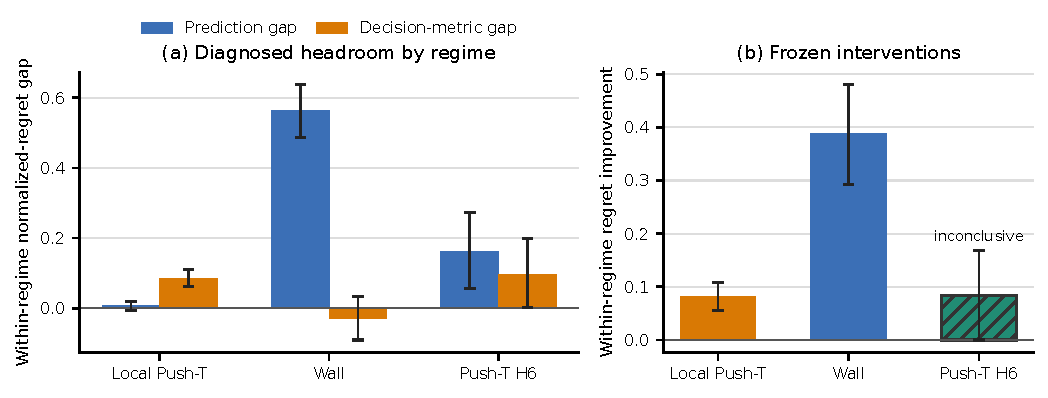
\includegraphics[width=0.88\textwidth]{figures/cross_regime_results.pdf}
  \caption{\textbf{Across-regime diagnosis and intervention.} (a) Candidate-matched prediction and decision-metric headroom. (b) Mean regret improvement from the diagnosis-selected intervention. Error bars are 95\% paired bootstrap CIs over states or episodes. The hatched H6 result is directionally positive but statistically inconclusive because its CI crosses zero.}
  \label{fig:results}
\end{figure*}

\subsection{Local Push-T: a decision-metric bottleneck}

The ground-truth-latent and predicted-latent task readouts achieve state-level Spearman correlations of $0.696$ and $0.689$ with simulator cost; their normalized regrets are $0.0289$ and $0.0360$. Consequently, prediction headroom is only $0.0071$ (95\% CI $[-0.0051,0.0198]$). Under the same predicted futures, replacing the readout with latent L2 exposes a much larger metric gap of $0.0851$ $[0.0608,0.1109]$. Proposal headroom is $0.0074$. Under the frozen rule, this controlled local protocol is decision-metric limited.

The diagnosis-selected repair reduces regret from $0.1237$ with BF16 prediction and latent L2 to $0.0421$ with the task readout: an improvement of $0.0815$ $[0.0563,0.1079]$. Across states, 62\% improve, 21\% are unchanged, and 17\% are harmed. The FP32-predictor plus latent-L2 control improves regret by only $0.0017$, with a CI crossing zero. This supports the narrow statement that increasing predictor inference precision did not recover planning performance; FP32 is not evidence that every possible predictor improvement would fail.

The observed repair closely matches the prior metric gap, whereas the precision control aligns with the negligible prediction gap. This diagnosis-to-intervention agreement is the principal local Push-T result.

\subsection{Wall: an independent prediction bottleneck}

On 80 diagnosis states, prediction headroom is $0.5636$ $[0.4871,0.6373]$, metric headroom is $-0.0279$ with a CI crossing zero, and proposal headroom is $0.0333$. The same rule that diagnoses local Push-T as metric limited therefore diagnoses Wall as prediction limited. This counter-regime makes clear that the procedure is not constructed to declare latent L2 the bottleneck.

On 80 entirely new repair states, the pre-specified predictor repair reduces regret from $0.5561$ to $0.1670$, an improvement of $0.3891$ $[0.2930,0.4804]$. The wrong-layer metric repair improves regret by $0.0069$ $[-0.0489,0.0625]$. Full-trajectory latent MSE falls from $0.8564$ to $0.1999$.

Average prediction improvement is not sufficient for state-wise decision improvement. In a retained counterexample, one anchor's latent MSE improves while regret worsens from $0.215$ to $0.991$. This does not negate the aggregate repair; it bounds the claim: lower predictive error does not guarantee better action selection for every state. The Wall predictor repair uses one training seed, which limits claims about training variability.

\subsection{H6: bottleneck migration and metric--search coupling}

On the official H6 baseline trace, GT-readout, predicted-readout, and predicted-L2 mean regrets are $0.1724$, $0.3332$, and $0.4282$. Prediction headroom is therefore $0.1608$ $[0.0565,0.2725]$, exceeding metric headroom $0.0950$ $[0.0026,0.1978]$. The result is mixed---both gaps are positive---but prediction is the larger limitation under the frozen rule. This differs from the controlled local action slice: long 60-D sequences broaden the candidate family and accumulate model error.

Matched-budget baseline and task-readout CEM obtain regrets of $0.4974$ and $0.4131$. The scorer-repair improvement is $0.0843$ $[-0.00008,0.1684]$: 16 episodes improve, 9 are unchanged, and 5 worsen. Because the interval narrowly crosses zero, the result is \textbf{directionally positive but statistically inconclusive}, not a validated successful repair.

The adaptive traces explain why fixed-candidate attribution need not predict end-to-end gain exactly. Changing the scorer reduces within-trace selection gap but can redirect future proposals. In a retained H6 episode, the readout selects the simulator-best sequence in its own trace, yet search coverage degrades and normalized regret worsens from $0.4044$ to $1.0000$. Thus a better ranking rule on available candidates need not expose better candidates under adaptive search.
